{\centering\Large{\MakeUppercase{\capspace{solemn novena in preparation for the feast of the assumption of \\ the b.v.m.}}}\par}

\begin{enpars}

\rubrique{As the ministers enter:}
\halfbskipvspace
%%Immaculate Mary novena version

{\centering{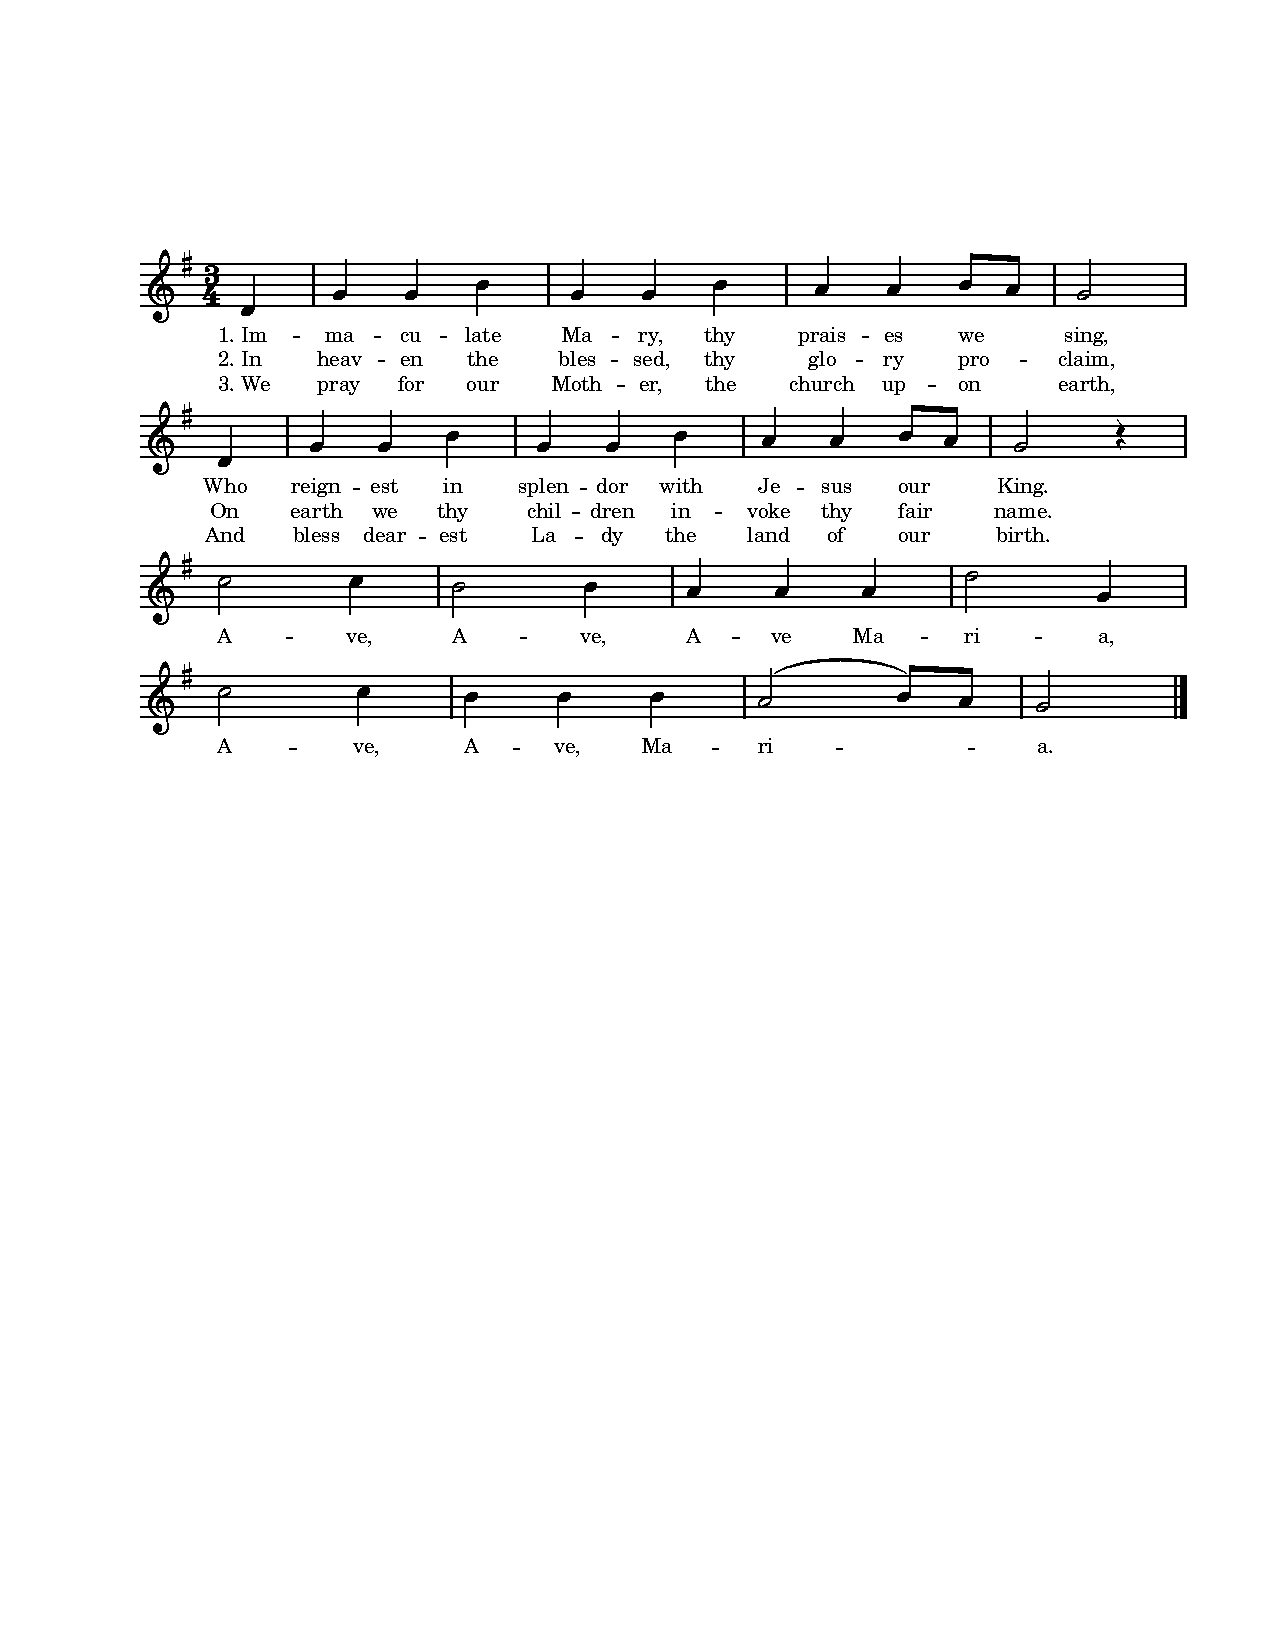
\includegraphics[scale=0.75,keepaspectratio]{immaculate_mary_american_novena_cropped}\par}}

\rubrique{The sermon is preached.}

\rubrique{After the sermon:}
%HHQ version at Mass has different end to 2nd verse in Worship II/III than version copied here
%{\centering{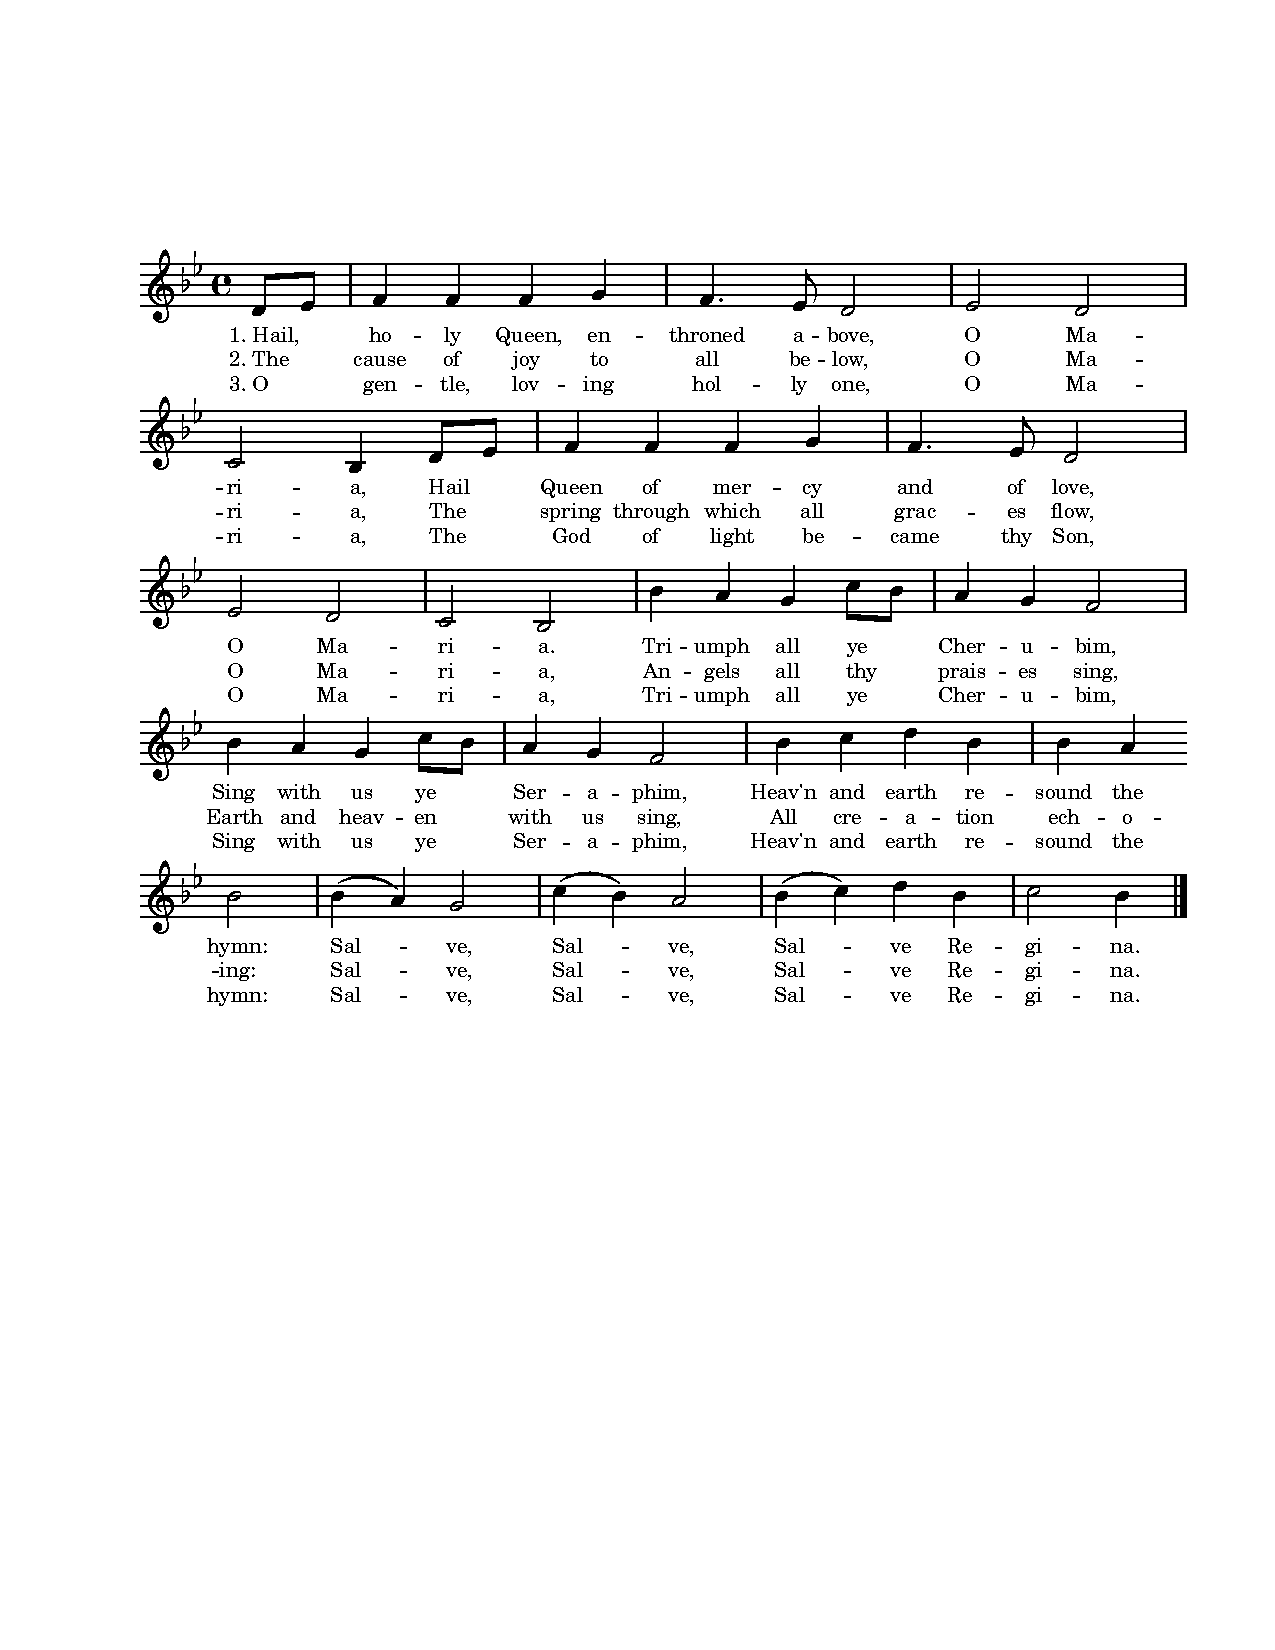
\includegraphics[scale=0.75,keepaspectratio]{hail_holy_queen_cropped}\par}}
{\centering{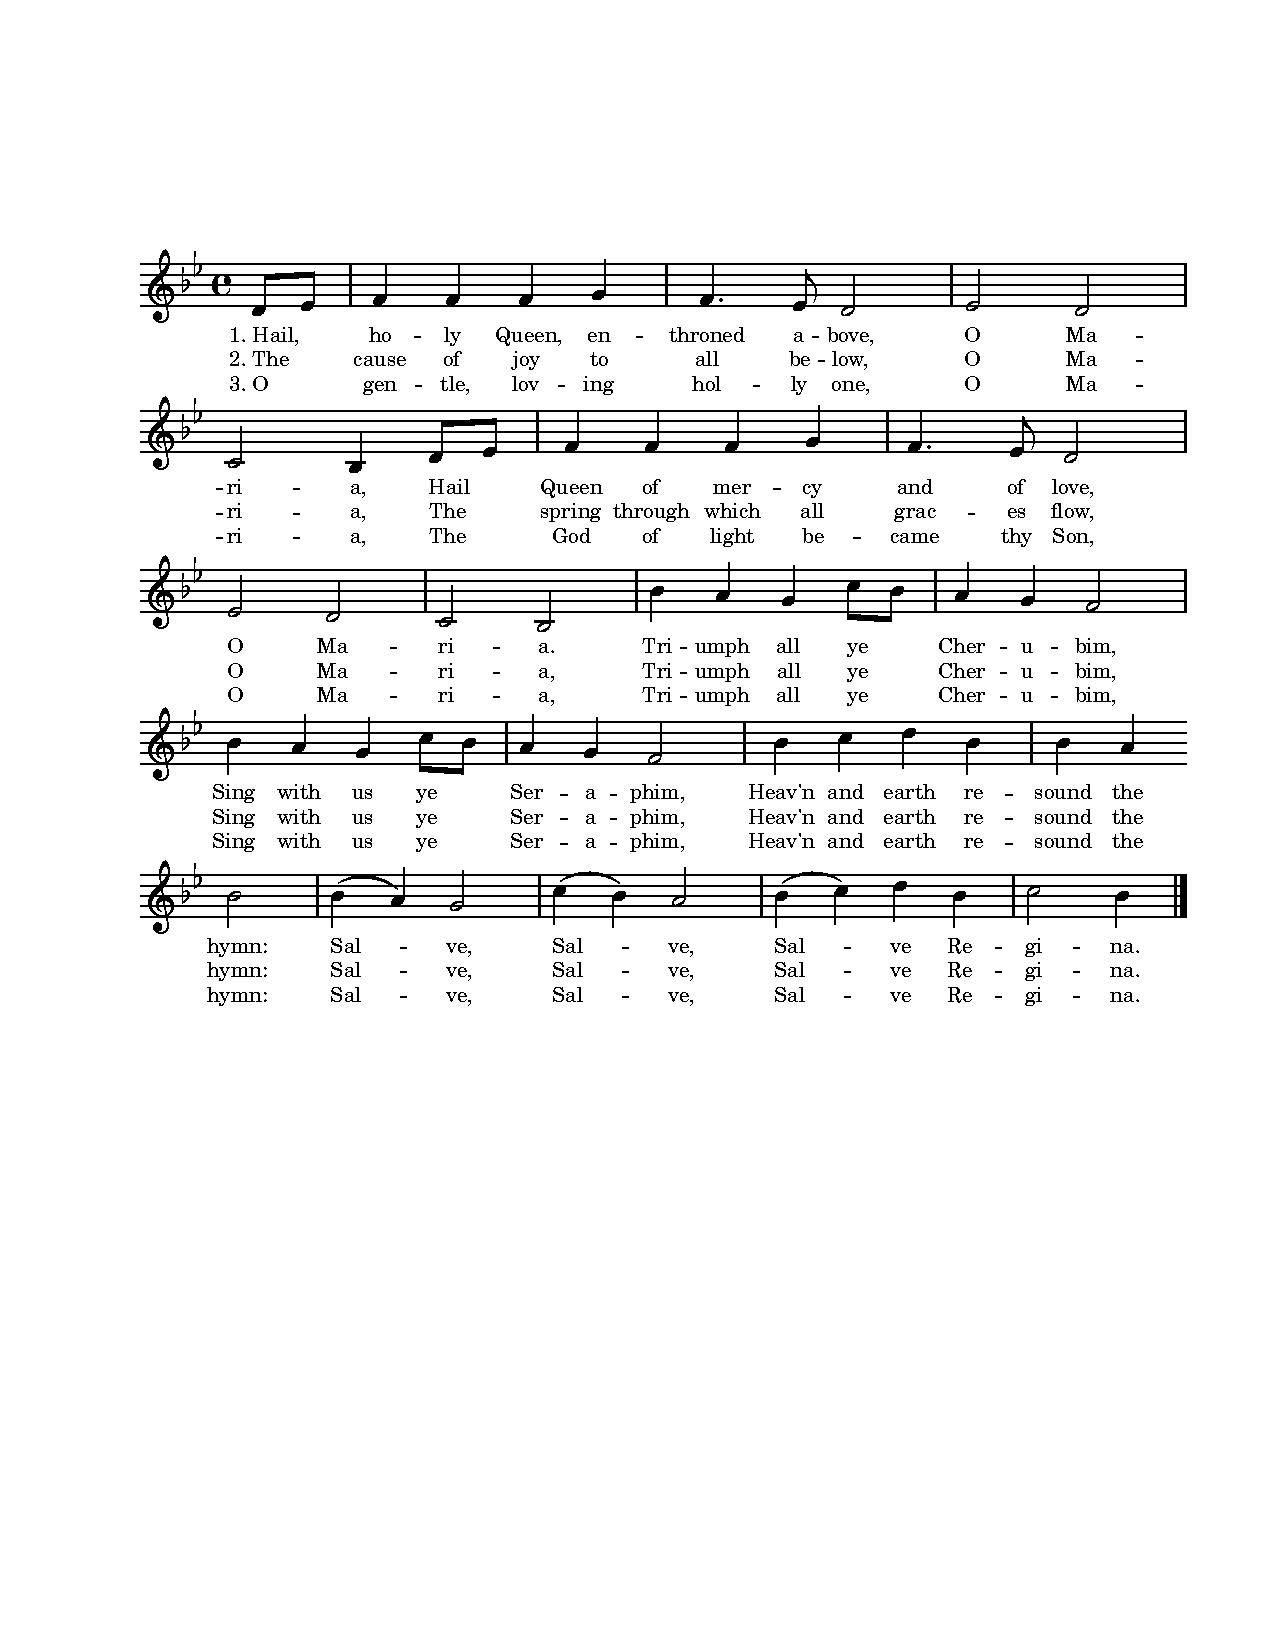
\includegraphics[scale=0.75,keepaspectratio]{hail_holy_queen_triumph_cropped}\par}}

\newpage
\rubrique{Then the Most Blessed Sacrament is exposed with \normaltext{O Salutáris, \pageref{M-o_salutaris_la_en}.}}

{\centering\large{\MakeUppercase{\capspace{novena prayer}}}\par}

\lettrine{O}{} most holy Virgin and my Mother, o Mary, * to thee who art the Mother of my Lord and the refuge of sinners,*  I have recourse today. * I render thee most humble homage * for all the graces which thou hast conferred upon me until now. * I love you, most aimiable Lady; * and for the love I bear thee, *  I promise to serve thee always, * and to do all in my power to make others love thee also. *  Dearest Mother, bring before the throne of thy beloved Son *  the prayers and intentions I ask during this novena:

\rubrique{Here mention your intentions. Please also pray for all who are present today. Pray for the intentions of our Holy Father the Pope, and for all the clergy. Pray also for the sick and the dying, and for the suffering souls in purgatory.}

\lettrine{I}{} place in thee all my hopes; * I confide my salvation to thy care. *  Accept me for thy servant and receive me under thy mantle, * o Mother of mercy. * And since thou art so powerful with God, *  deliver me from all temptations, *  or rather obtain for me the strength to triumph over them until death. *  Of thee I ask a perfect love for Jesus Christ. *  Through thee I hope to die a good death. *  O my Mother, by the love which thou bearest to God, *  I beseech thee to help me at all times, * especially at the last moment of my life. * Leave me not, I beseech thee, until I am safe in heaven, *  blessing thee and singing thy mercies for all eternity. * Amen.

\rubrique{Benediction of the Most Blessed Sacrament follows. \normaltext{Tantum ergo, ℣. Panem de cælo,} and collect \normaltext{Deus qui nobis,} \normaltext{\pageref{M-tantum_ergo_la_en}.}}

\rubrique{After Benediction of the Most Blessed Sacrament, the Divine Praises are recited, \normaltext{\pageref{M-divine_praises}.}}

\rubrique{At the reposition, \normaltext{Holy God, We Praise Thy Name, \pageref{M-holy_god_we_praise_thy_name}.}}

\rubrique{Then \normaltext{Salve Regína,} simple tone, \normaltext{℣. Ora pro nobis,} and collect \normaltext{Omnípotens, \pageref{M-an_salve_regina_simple_tone_solesmes}.}}

\rubrique{As the ministers retire:}
%%Sing of Mary
{\centering{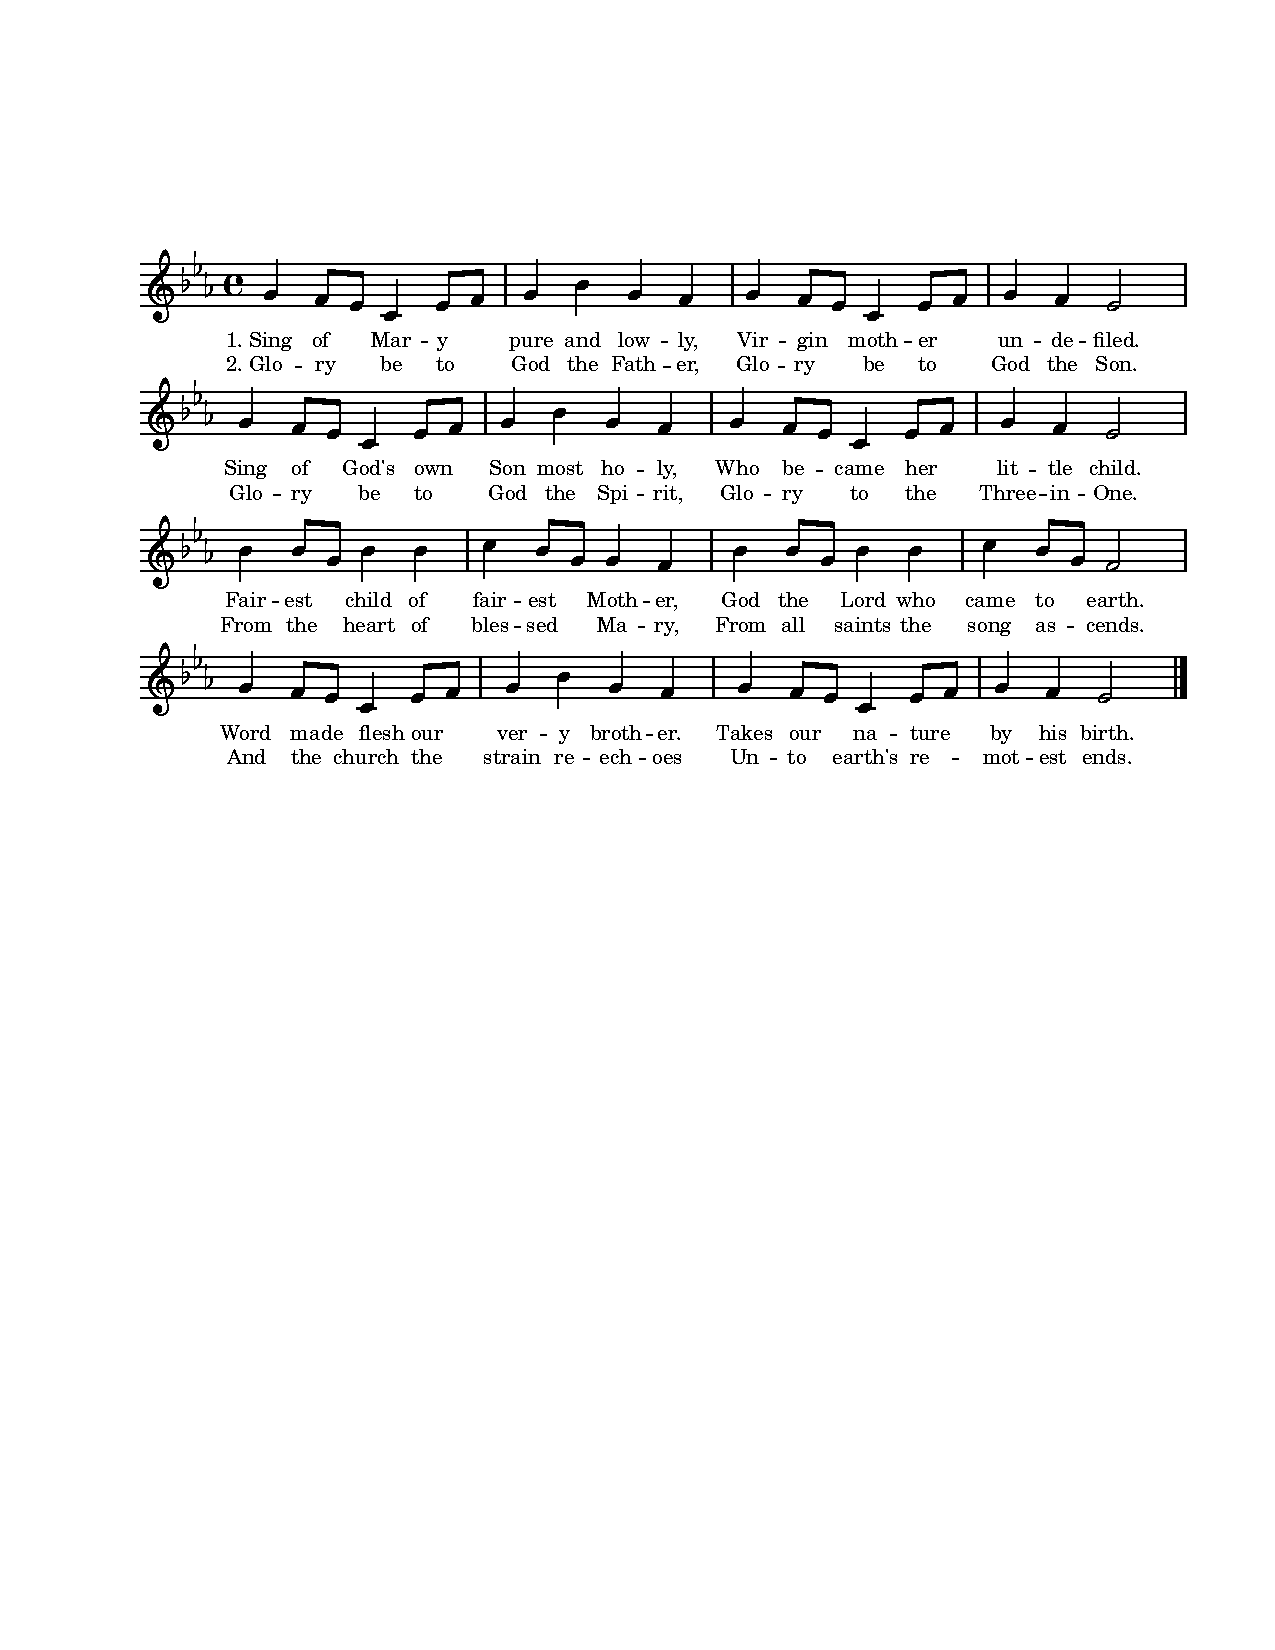
\includegraphics[scale=0.75,keepaspectratio]{sing_of_mary_pure_and_lowly_melody_cropped}\par}}
\end{enpars}